\documentclass{bioinfo}
\usepackage{url}

\usepackage[british,english]{babel}
\usepackage{mathpazo}
\usepackage{color}
\definecolor{deepblue}{rgb}{0,0,0.5}
\definecolor{deepred}{rgb}{0.6,0,0}
\definecolor{deepgreen}{rgb}{0,0.5,0}

\usepackage{listings}
\usepackage{setspace}

\definecolor{Code}{rgb}{0,0,0}
\definecolor{Decorators}{rgb}{0.5,0.2,0.2}
\definecolor{Numbers}{rgb}{0.5,0,0}
\definecolor{MatchingBrackets}{rgb}{0.25,0.5,0.5}
\definecolor{Keywords}{rgb}{0,0.6,0}
\definecolor{self}{rgb}{0,0,0}
\definecolor{Strings}{rgb}{0,0.63,0}
\definecolor{Comments}{rgb}{0,0.63,1}
\definecolor{Backquotes}{rgb}{0,0,0}
\definecolor{Classname}{rgb}{0,0,0}
\definecolor{FunctionName}{rgb}{0,0,0}
\definecolor{Operators}{rgb}{0,0,0}
\definecolor{Background}{rgb}{1,1,1}

\lstnewenvironment{python}[1][]{
\lstset{
%numbers=left,
numberstyle=\footnotesize,
numbersep=1em,
xleftmargin=1em,
framextopmargin=2em,
framexbottommargin=2em,
showspaces=false,
showtabs=false,
showstringspaces=false,
%frame=l,
tabsize=4,
% Basic
basicstyle=\ttfamily\small\setstretch{1},
backgroundcolor=\color{Background},
language=Python,
% Comments
commentstyle=\color{Comments}\slshape,
% Strings
stringstyle=\color{Strings},
morecomment=[s][\color{Strings}]{"""}{"""},
morecomment=[s][\color{Strings}]{'''}{'''},
% keywords
morekeywords={import,from,class,def,for,while,if,is,in,elif,else,not,and,or,print,break,continue,return,True,False,None,access,as,del,except,exec,finally,global,import,lambda,pass,print,raise,try,assert},
keywordstyle={\color{Keywords}\bfseries},
% additional keywords
morekeywords={[2]@parametric},
keywordstyle={[2]\color{Decorators}\slshape},
emph={self},
emphstyle={\color{self}\slshape},
%
}}{}


\usepackage[T1]{fontenc}
% \usepackage[latin9]{inputenc}
\usepackage{float}
\usepackage{amsmath}
\usepackage{graphicx}
\usepackage{setspace}
\usepackage{amssymb}
\usepackage{natbib}
\usepackage[title]{appendix}
\usepackage{siunitx}
\usepackage{chngcntr}
\usepackage{algorithmic}
\renewcommand{\algorithmicrequire}{\textbf{Input:}}
\renewcommand{\algorithmicensure}{\textbf{Output:}}

\usepackage{multirow}
\usepackage{rotating}
\usepackage{hyperref}

\makeatletter
\newfloat{algorithm}{H}{loa}[section]
\floatname{algorithm}{Algorithm}
\counterwithout{algorithm}{algorithm}
\def\argmin{\mathop{\operator@font arg\,min}} 
\def\argmax{\mathop{\operator@font arg\,max}} 
\makeatother

\copyrightyear{}
\pubyear{}

\begin{document}
\firstpage{1}

\title[QuickBundles]{Dipy, a library for the analysis of diffusion MRI data}

\author[Garyfallidis, Brett, Amirbekian, Rokem,  van der Walt, Descoteaux, 
Nimmo-Smith]{Eleftherios~Garyfallidis\,$^{1,2,*}$, Matthew~Brett\,$^{3}$,
  Bago~Amirbekian\,$^{4}$, Ariel~Rokem\,$^{5}$, Stefan~van der Walt\,$^{7}$, Maxime~Descoteaux\,$^{2}$, Ian~Nimmo-Smith\,$^{6}$ and Dipy~Contributors $^{8}$\footnote{to whom correspondence should be addressed. e-mail: garyfallidis@gmail.com}}

\address{\,$^{1}$University of Cambridge, Cambridge, UK\\
  \,$^{2}$University of Sherbrooke, Sherbrooke, CA\\ 
  \,$^{3}$University of California, Henry H. Wheeler, Jr. Brain Imaging Center, Berkeley, CA.\\
  \,$^{4}$University of California, San Francisco, CA, USA\\    
  \,$^{5}$Stanford University, Stanford, CA, USA\\
  \,$^{6}$MRC Cognition and Brain Sciences Unit, Cambridge, UK\\
  \,$^{7}$Stellenbosch University, Stellenbosch, South Africa\\
  \,$^{8}$http://dipy.org/developers.html  
  }

\history{}

\editor{}

\maketitle

\begin{abstract}
\noindent

Diffusion Imaging in Python (Dipy) is a free and open source software
project for the analysis of data from diffusion magnetic resonance
imaging (dMRI) experiments. DMRI is an application of MRI that can be
used to measure the micro-structure of the white matter in the human
brain in vivo. It utilizes the application of directionally oriented
magnetic gradients to estimate diffusion in different directions and
locations in the brain non-invasively. Many methods have been developed
to model the local configuration of nerve fibers in the white matter
based on this information and to infer the trajectory of fascicles
connecting different parts of the brain. However, no single open source
software platform gathers implementations of all these different
methods, where they can be easily understood and compared. Dipy aims to
provide transparent implementations for all the different steps of dMRI
analysis with a relatively uniform API.

Dipy implements classical signal reconstruction techniques, such as the
diffusion tensor model (Basser et al., 1994) and deterministic fiber
tractography (Mori et al., 1999). In addition, it implements cutting
edge novel reconstruction techniques, such as generalized Q imaging (Yeh
et al., 2010) and diffusion spectrum imaging with deconvolution
(Canales-Rodriguez et al. 2010), as well as methods for probabilistic
tracking (Berman et al., 2008) and unique methods for tractography
clustering (Garyfallidis et al., 2012). Many additional utility
functions, to calculate various statistics of dMRI data, visualization
functions, as well as file-handling routines exist to assist in the
development of novel techniques.
 
Dipy makes use of the scientific software for neuroimaging that exists
in python (e.g. nibabel), as well as python tools for numerical
processing (numpy), visualization (python-vtk), high performance
computation (cython) and software testing (nose).

In contrast to many other scientific software projects, dipy is not
being developed by a single research group. Rather, it is an open
project that encourages contributions from any scientist-developer
through the github Pull Request mechanism and open discussions on github
and on the project mailing list. Consequently, dipy has today an
international team of contributors, spanning 6 different academic
institutions in 4 countries and 3 continents, and still growing
(http://dipy.org).

\section{Keywords:} Python, Diffusion MRI, Diffusion Tensor model,
Deconvolution, Medical imaging, Open source software, Deterministic
tractography, Probabilistic tractography, Visualisation.

\end{abstract}

\section{Skeleton}

Here is a possible outline for the paper:

\begin{verbatim}
Short overview of other dMRI analysis tools
Philosophy/Mission
General Design Aspects
How we work (git/github etc)
File Formats 
Preprocessing
   Eddy currents?
   Denoising?
Reconstruction
   DTI 
   DSI
   QBall
   Spherical Deconvolution 
Tracking
   Deterministic
   Probabilistic
Post-tracking
   Segmentation
   Track_counts
   Track Lengths & other statistics
   Connectivity matrix?
Conclusions
\end{verbatim}


\section{Introduction}

\emph{Diffusion MRI} (dMRI) \citep{stejskal-tanner:65, lebihan-breton:85,merboldt-hanicke-etal:85, taylor-bushell:85, callaghan:91} is the principal non-invasive method that provides information about the directional structure of neuronal pathways found in the white matter and other body tissue with fiber-like structure. dMRI acquires one or 
more $T_{2}$ reference images, and a collection of diffusion-weighted images that attenuate the $T_{2}$ signal according to the amount of diffusion along prescribed gradient directions \citep{behrens-johansen-berg:09, jones:10}. 

Because of its unique capability to depict structural connectivity, during the last 10 years, dMRI had an increasing popularity with more than five thousand papers published according to PubMed only for 2012. This popularity is also evident from the large number of software tools available for the analysis of diffusion weighted images. Most of these tools are written in C/C++: 3D Slicer \citep{pieper:06}, AFNI \citep{cox-afni:12}, MITK \citep{fritzsche-mitk:12}, BrainVoyager QX \citep{goebel-brainvoyager:12}, DTI-Query/Quench \citep{sherbondy:05}, FreeSurfer \citep{fischl-freesurfer:12}, FSL-FDT \citep{smith-fdt:04}, MedInria \citep{toussaint-souplet-etal:07}, MRtrix \citep{Tournier2012}, Diffusion Toolkit/Trackvis \citep{wang-diffusion-toolkit:07}, and FiberNavigator \citep{vaillancourt:11, chamberland:13}, R: TractoR \citep{ clayden-TractoR:11}, Java: Camino \citep{Cook2006} and Matlab: ExploreDTI \citep{leemans-exploredti:09}. 

Dipy which stands for \textit{Diffusion Imaging in Python} is the first collective effort to create a diffusion MRI analysis library in Python language. Python is a general purpose, object-oriented programming language which emphasizes in code readability. Code readability, a key feature of Python enables people who are not necessarily programming gurus to understand and extend the underlying code in a simple and comprehensive manner. We think that this is a powerful asset for the design of the next generation of medical imaging analysis tools. In the past we found that many researchers were using available tools without understanding the underlying details, often because the details were hidden from the users. Dipy tackles this problem be being free, open source (BSD license), simple and well documented. 

Dipy is built on top of production-ready high-performance Python libraries. Primarily, Dipy uses the Numpy Array \citep{van_numpy:11} as its core structure. Numpy arrays are the standard representation for numerical data in Python and enable efficient implementation of numerical computations allowing vectorizing calculations, avoiding copying data in memory, and minimizing operations. The Numpy Array is part of a more general numerical library (Numpy\footnote{\url{http://numpy.org}}) which can be used for example for matrix, tensor and linear algebra operations. Dipy also depends on Scipy\footnote{\url{http://scipy.org}} (a superset of Numpy) for nonlinear optimization and other volumetric operations. Cython\footnote{\url{http://cython.org}} is used in rare cases when both standard Python and Numpy/Scipy are not efficient enough for the task at hand. Cython interprets Python code into plain C performance by adding static type declarations. The last hard dependency for Dipy is Nibabel\footnote{\url{http://nipy.org/nibab}} which is used for loading and saving medical imaging datasets.

Furthermore, Dipy recommends the use of IPython\footnote{\url{http://ipython.org}} for interacting with the datasets and debugging the code, the IPython notebook for teaching, Matplotlib\footnote{\url{http://matplotlib.org}} for plotting 2D/3D datasets and Python-VTK\footnote{\url{http://vtk.org}} for more advanced 3D interactive visualization. Nonetheless, these are optional dependencies and they are not required for the standard use of Dipy.

\citep{perez_ipython:07}, \citep{perez_python:11}, \citep{mckinney_python:12}, 




\begin{python}
from dipy.viz import fvtk
ren = fvtk.ren()
class Test(object):
  def __init__(self, a):
    pass

@parametric
def f(x):
  return x**2
for i in range(10):
  print f(i)
\end{python}


\section{Philosophy and Mission}

Someone will write this.

\section{LaTex Formatting Stuff}

This is to show how graphics (EPS) files are included. We use EPS for
speed. The first one is spread across both columns, and the second one
is just in a single column:

\begin{figure*}
\centerline{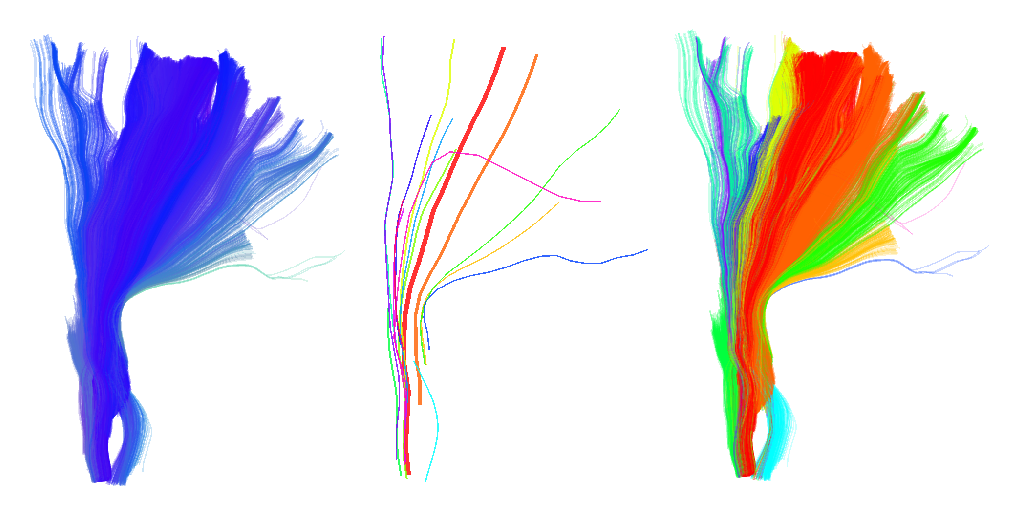
\includegraphics[width=160mm]{Figures/Fig_4_cst_simplification_relabeled_triple.eps}}
\caption{This is the figure caption - and a label to refer to it in the text \label{Fig:big_picture}}
\end{figure*}

When we want to refer to this figure we use the label (see
Fig.~\ref{Fig:big_picture}).

\begin{figure}
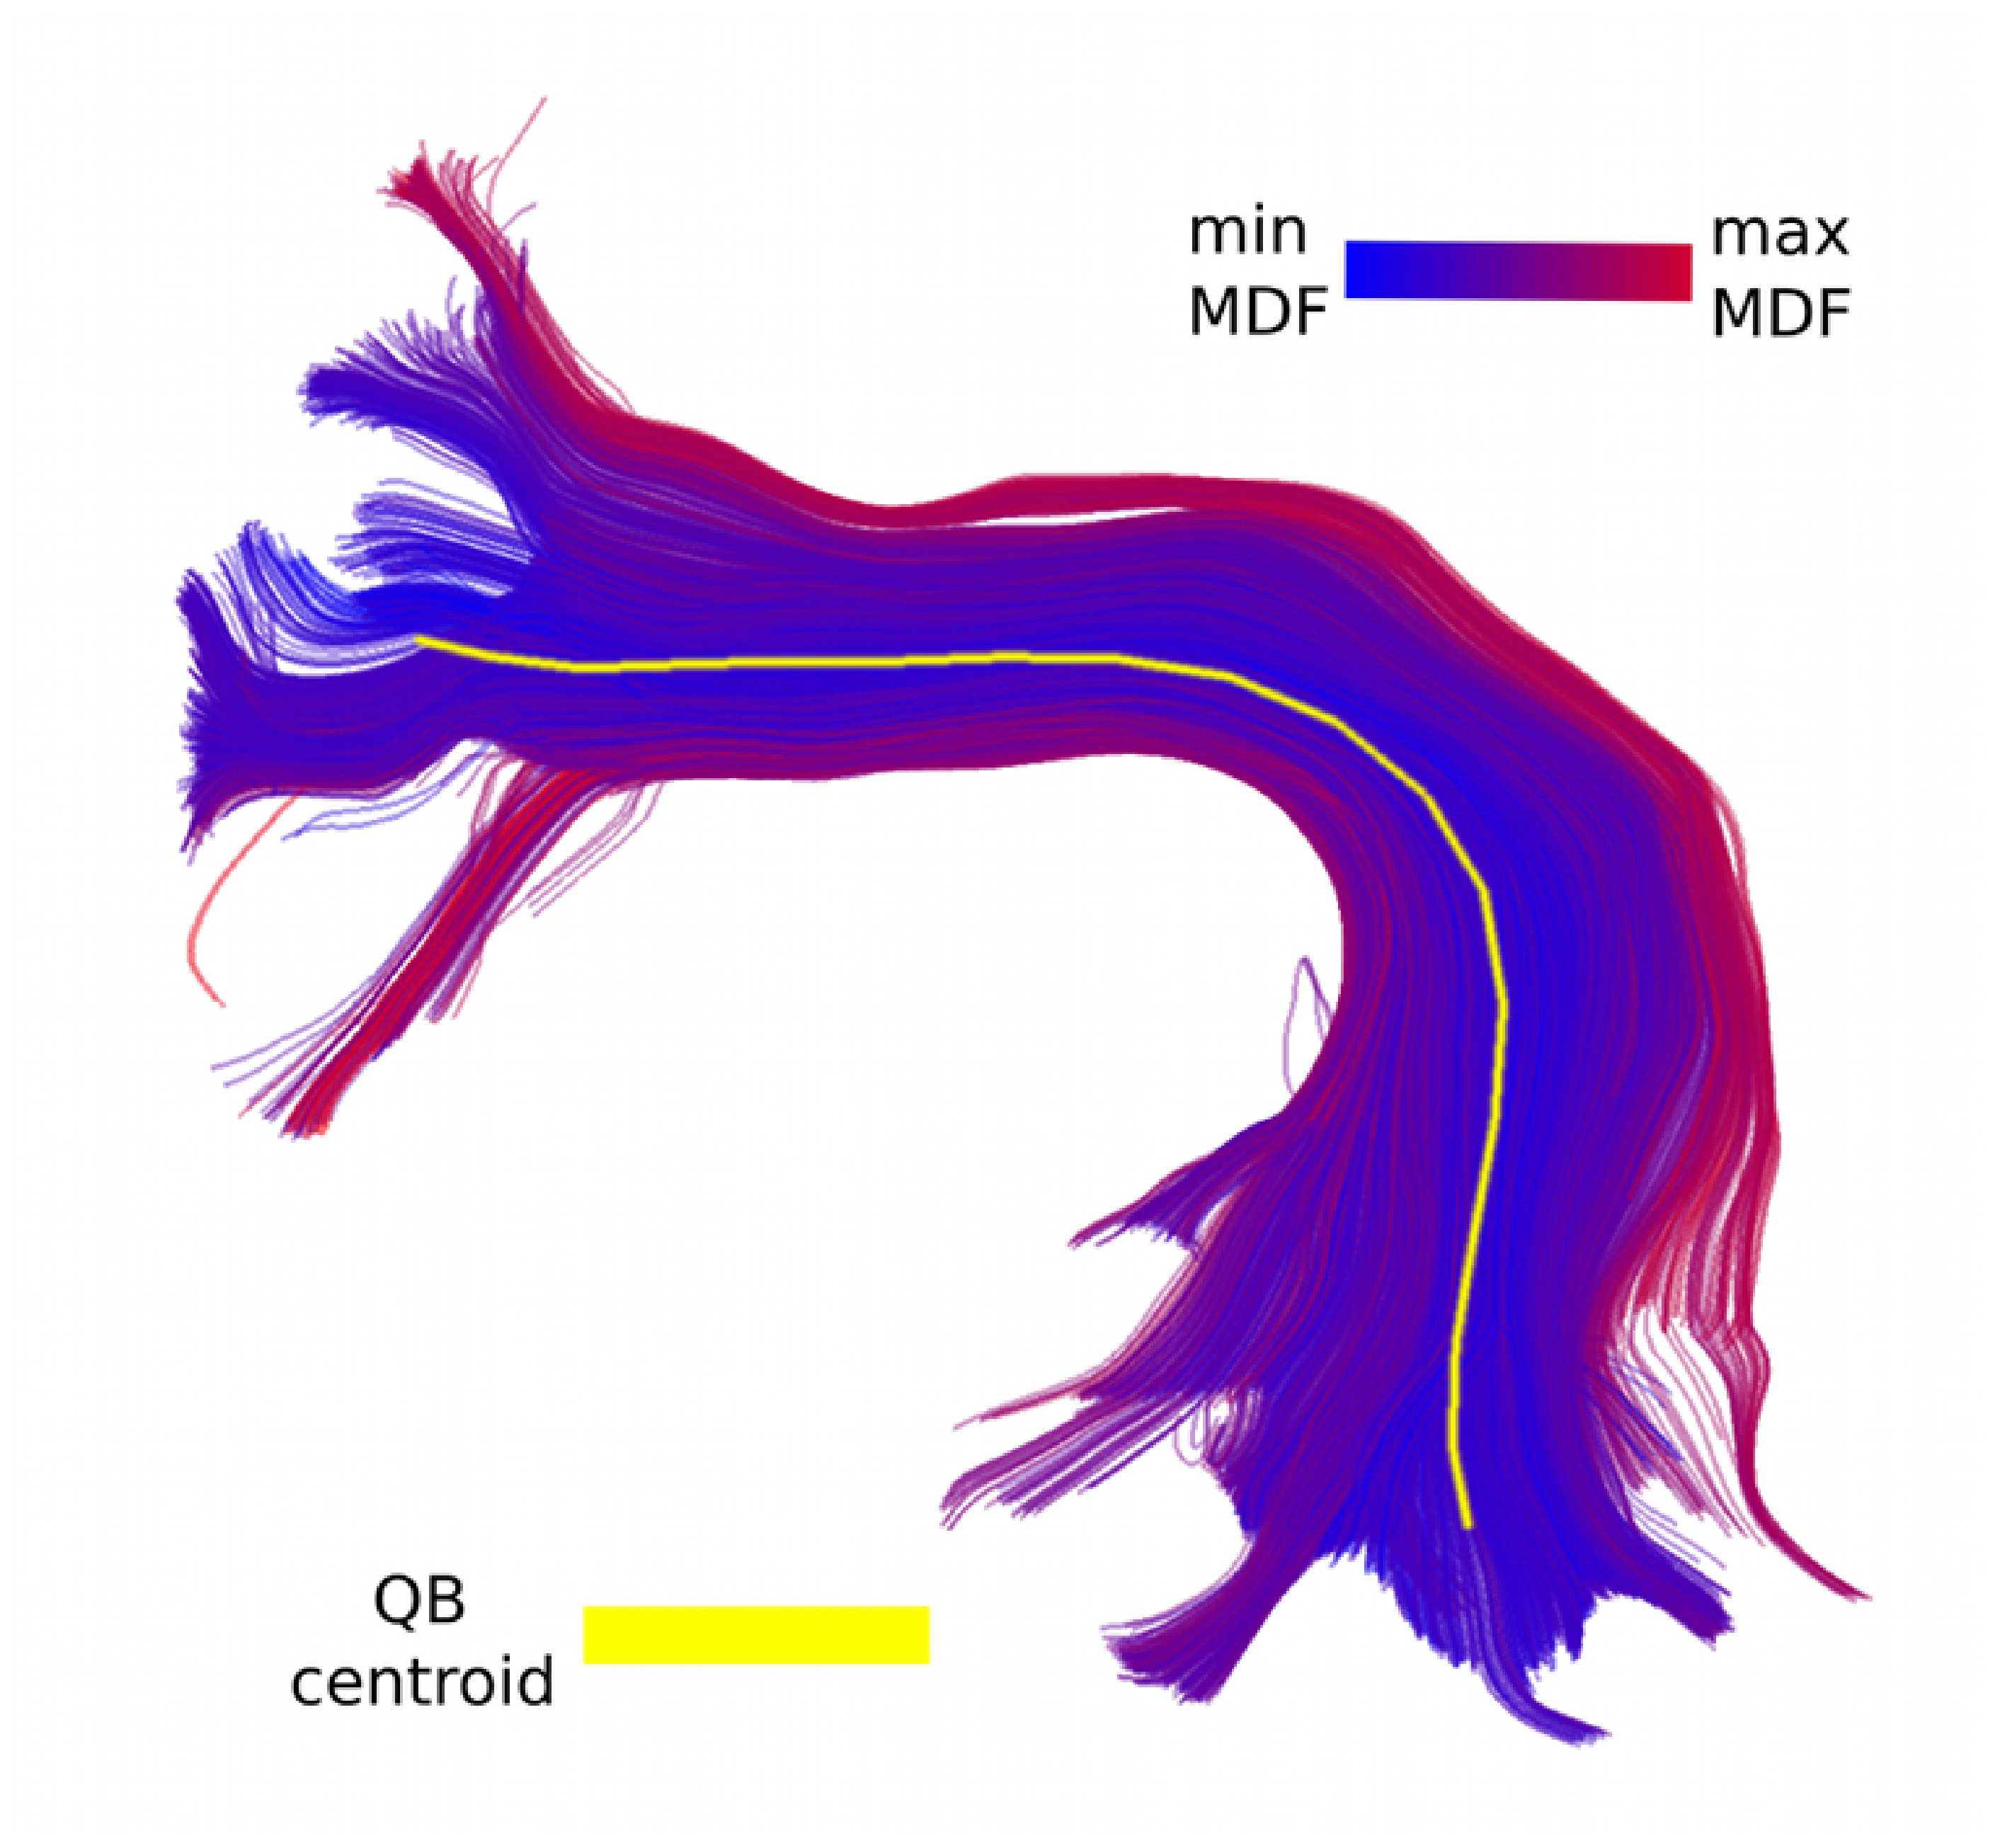
\includegraphics[scale=0.15]{Figures/Fig_11_MDF_arcuate}
\centering{}
\caption{Color coding shows MDF distances from QB centroid to every
  other track in the bundle.\label{Fig:little_picture}}
\end{figure}

Here are some displayed equations (see Eq.~\ref{eq:direct_flip_distance}):
\begin{eqnarray}
  d_{\textrm{direct}}(s, t) = d(s, t) & = & \frac{1}{K}\sum_{i=1}^{K}|s_{i}-t_{i}|,\nonumber\\
  d_{\textrm{flipped}}(s, t) & = & d(s,t^F) = d(s^F,t),\nonumber\\
  \textrm{MDF}(s, t) & = & \min(d_{\textrm{direct}}(s, t), d_{\textrm{flipped}}(s, t))\label{eq:direct_flip_distance}.
\end{eqnarray}

Inline mathematics goes like this: $\frac{1}{K}\sum_{i=1}^{K}|s_{i}-t_{i}|$

Here we have an example of a table (see Table~\ref{Table_1}).

\begin{table}[th] \processtable{QB centroids performance compared with
random subsets\label{Table_1}} {\begin{tabular}{rrrr} %\hline Thresholds &
Comparison & Coverage \% (s.d.) & Overlap (s.d.) \\ \hline
\multirow{2}{*}{$10$~mm/$10$~mm} & QB Centroids & 99.96 (0.007) & 2.44
(0.08)\\ & Random & 90.49 (0.41) & 6.16 (0.55)\\ \hline
\multirow{2}{*}{$20$~mm/$20$~mm} & QB Centroids & 99.99 (0.004) & 3.54
(0.18)\\ & Random & 95.86 (0.62) & 6.81 (0.93)\\ \hline
\end{tabular}}{}
\end{table}

References go like this: in parentheses
\citep{Garyfallidis_thesis,Mori1999}, and in running text
\citet{Garyfallidis_thesis}.

\section*{Acknowledgments}
Who do we need to acknowledge?

\section*{Disclosure/Conflict-of-Interest Statement}
Is it true that there are no conflicts of interest relating to this
work?

\selectlanguage{british}%
\bibliographystyle{apalike2}
%\bibliographystyle{plainnat}
%\bibliographystyle{IEEEabrv, IEEEtran}
%\bibliographystyle{IEEEtran}
%\bibliographystyle{elsarticle-harv}
\selectlanguage{english}
\bibliography{scilBibTex}

\end{document}
